\documentclass[12pt, a4paper ]{article}
\usepackage[T1]{fontenc}
\usepackage{a4wide}
\usepackage[english]{babel}
\usepackage[utf8]{inputenc}
\usepackage{eurosym}%signe euro 
%\usepackage{graphicx}
\usepackage{amsmath}
\usepackage{lipsum,multicol}
\usepackage{verbdef}
\usepackage[colorlinks,bookmarks=false,linkcolor=black,urlcolor=blue, citecolor=black]{hyperref}
\usepackage[top=3cm, bottom=3cm, left=2cm, right=2cm]{geometry}
\usepackage{float}
\usepackage{wrapfig}
\usepackage{listings}
\usepackage[table]{xcolor}
\usepackage{caption}
\usepackage{subcaption}
\usepackage{tabularx}
\usepackage{enumitem}
\usepackage[utf8]{inputenc}
\usepackage[printonlyused]{acronym} 
\usepackage{amsmath}
\usepackage{multirow}
\usepackage{tikz}
\usepackage{circuitikz}
\usepackage{svg}
\usetikzlibrary{arrows,automata}
%en-tete et pied de page



\begin{document}



\section{Introduction}
This part shows the $GPW$ minimum reachable with actual available resources in Switzerland while minimizing the $TOTEX$.
The optimizer is able to compute scenarios until a $GWP_{min}$ at $7693.00 ktCO_2/y$ for which the $TOTEX$ is $30224.95 MCHF/y$.
This represents a $GWP$ improvement of X\% to the detriment of the $TOTEX$ which increases of Y\%.
In this scenario, nuclear power and Natural gas CCS take a prominent place. Renewable energies like Geothermal, wind, and solar grow. 
However, if Switzerland wishes to abandon its nuclear power plants, it can then go down to a $GWP$ of $10422.00 ktCO_2/y$ replacing this lack of energy with Natural gas CCS. 
In this case, as Natural gas CCS is more expensive than nuclear, the $TOTEX$ reaches $27262.40 MCHF/y$.

\begin{figure}[H]
    \centering
    \begin{subfigure}[b]{0.45\textwidth}
        \centering
        \includegraphics[width=1\textwidth]{data/LOW_GWP_nuc.png}
        \caption{Using nuclear}
    \end{subfigure}
    \begin{subfigure}[b]{0.45\textwidth}
        \centering
        \includegraphics[width=1\textwidth]{data/LOW_GWP_wnuc.png}
        \caption{Without nuclear}
    \end{subfigure}
    \caption{Sankey diagrams of power repartition with the $GWP_{min}$}
    \label{fig:sankey1}
\end{figure}
\begin{figure}[H]
    \centering
    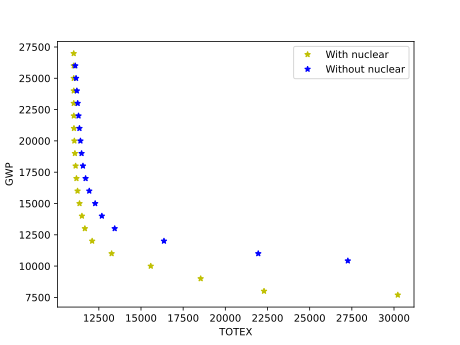
\includegraphics[width=.8\textwidth]{data/TOTEX_GWP.eps}
    \caption{caption}
    \label{fig:GWP_vs_TOTEX}
\end{figure}
Figure \ref{fig:sankey1} show the division of energies computing with those $GWP_{min}$.
Figure \ref{fig:GWP_vs_TOTEX} represent the evolution of the $TOTEX$ with different $GWP$ objective. It shows that wanting to reach the $GWP_{min}$ is not a good solution. Indeed, $TOTEX$ grows exponentially.
It, therefore, makes sense to choose a $GWP$ higher than the $GWP_{min}$.



\end{document}
